\documentclass[titlepage]{scrartcl}
\usepackage{enumitem}
\usepackage[british]{babel}
\usepackage[style=apa, backend=biber]{biblatex}
\DeclareLanguageMapping{british}{british-apa}
\usepackage{url}
\usepackage{float}
\usepackage[labelformat=empty]{caption}
\restylefloat{table}
\usepackage{perpage}
\MakePerPage{footnote}
\usepackage{abstract}
\usepackage{graphicx}
% Create hyperlinks in bibliography
\usepackage{hyperref}
\usepackage{amsmath}

\usepackage[T1]{fontenc}
\usepackage[utf8]{inputenc}
\usepackage{blindtext}
\setkomafont{disposition}{\normalfont\bfseries}

\graphicspath{
    {./resources/},
}
\addbibresource{~/Documents/library.bib}

\DeclareSourcemap{
    \maps{
        \map{ % Replaces '{\_}', '{_}' or '\_' with just '_'
            \step[fieldsource=url,
                  match=\regexp{\{\\\_\}|\{\_\}|\\\_},
                  replace=\regexp{\_}]
        }
        \map{ % Replaces '{'$\sim$'}', '$\sim$' or '{~}' with just '~'
            \step[fieldsource=url,
                  match=\regexp{\{\$\\sim\$\}|\{\~\}|\$\\sim\$},
                  replace=\regexp{\~}]
        }
    }
}

\newsavebox{\abstractbox}
\renewenvironment{abstract}
  {\begin{lrbox}{0}\begin{minipage}{\textwidth}
   \begin{center}\normalfont\sectfont\abstractname\end{center}\quotation}
  {\endquotation\end{minipage}\end{lrbox}%
   \global\setbox\abstractbox=\box0 }

\usepackage{etoolbox}
\makeatletter
\expandafter\patchcmd\csname\string\maketitle\endcsname
  {\vskip\z@\@plus3fill}
  {\vskip\z@\@plus2fill\box\abstractbox\vskip\z@\@plus1fill}
  {}{}
\makeatother

\DeclareCiteCommand{\citeyearpar}
    {}
    {\mkbibparens{\bibhyperref{\printdate}}}
    {\multicitedelim}
    {}

% MATLAB Code block stuff...
\usepackage{color}
\usepackage{listings}

\definecolor{dkgreen}{rgb}{0,0.6,0}
\definecolor{gray}{rgb}{0.5,0.5,0.5}

\lstset{language=Matlab,
   keywords={break,case,catch,continue,else,elseif,end,for,function,
      global,if,otherwise,persistent,return,switch,try,while},
   basicstyle=\ttfamily,
   keywordstyle=\color{blue},
   commentstyle=\color{gray},
   stringstyle=\color{dkgreen},
   numbers=left,
   numberstyle=\tiny\color{gray},
   stepnumber=1,
   numbersep=10pt,
   backgroundcolor=\color{white},
   tabsize=4,
   showspaces=false,
   showstringspaces=false}

\begin{document}
\title{ECS732U --- Reat-time DSP}
\subtitle{\LARGE{Assignment 3}}
\author{Sam Perry --- ec16039}

\maketitle

\section{Overview}
This report presents a real-time PCG heart sound segmentation algorithm,
implemented for the Bela DSP processor. The project is based on previous work
by Liang et.\ al~\citeyearpar{Liang1997}. The aim was to create robust
real-time implementation of the heart sound segmentation algorithm in order to
allow for future development in areas such as heart sound classification.
Focus is placed on the accuracy of estimation and the robustness of the
detection algorithm across a range of PCG signals. This is measured using a PCG
dataset provided for the Physionet 2016 Cardiology Challenge
dataset~\parencite{Physionet2016}.  Segmentations produced by prototype systems
are compared to a pre-existing system proposed by Springer et.\
al~\citeyearpar{Springer2016} (currently considered the state of the art for
offline PCG signal segmentation).

\section{Background}
The analysis of phonocardiogram (PCG) data has shown promise in the field of
cardiology, providing a non-invasive, audio based alternative to similar
analysis methods such as the Electro-cardiogram (ECG). The effective
segmentation of PCG data is important for analysis of the signal as it
seperates significant phases of the cardiac cycle (the first and second heart
sounds). This segmentation data has been shown to be useful in areas such as
heart abnormality detection as described as part of the Physionet Challenge.

\section{Prototypes}
The aim of this project was to convert a pre-existing segmentation algorithm
from the offline version presented by Liang et.\ al to a real-time version
capable of running on a finite resource system such as the Bela board. The
algorithm was chosen for it's relative simplicity, as other algorithms tend to
adopt more complex machine learning based approaches, such as that presented by
Spirnger.\\

At the outset of this project, it was not certain that an effective
implementation would be possible, and even less so if it would be possible to
maintain the degree of accuracy described in previous research. For this
reason, the project was developed by first implementing two prototype
implementations in Python, in order to test the various elements and allow for
iterative evaluation of performance as the project progressed.

\subsection{Offline Python Implementation}
Initially an offline implementation of the algorithm was developed, aiming to
reproduce the algorithm presented as faithfully as possible. This would focus
on achieving the highest segmentation accuracy possible.\\
Following the method presented, the algorithm consists of the following stages:
\begin{enumerate}
    \item Pre-processing
    \item Feature Extraction
    \item Peak Picking
    \item Peak Processing
\end{enumerate}
\subsubsection{Pre-processing}
In order to filter out noise and reduce signal data, the paper suggests that
signals be decimated to remove all content above approximately 800Hz. As the
dataset used had already been processed to a similar degree, this was not
necessary in code, but should be considered for any future testing on other
datasets.
Normalisation of audio to it's absolute maximum was applied to bring all
signals up to a standard level:
$$
x_{norm}(k) = \frac{x(k)}{\max\limits_{i}(|x(i)|)}
$$
\subsubsection{Feature Extraction}
Average shannon energy is used for it's attenuation of low and high intensity
signal, allowing for the accentuation of medium intensity signal where heart
sounds are most likely to be. This is calculated as follows:
$$
E_s = -1/N\cdot\sum_{i=1}^{N}x^{2}_{norm}(i)\cdot\log x^{2}_{norm}(i)
$$
Windows were set to 0.02ms with a 50\% overlap as suggested.
The resulting analysis is illustrated in figure~\ref{OfflineShanEngy}
This shows the clear relationship between heart beats and spikes in energy

\subsubsection{Peak Picking}
Having generated an envelope for the signal, peaks must then be picked to
provide initial candidates for segmentation. This was achieved through the
adaptation of a peak picking algorithm~\parencite{PeakUtils}, adapted to suit the
suggested picking of a single peak per threshold overshoot. This is illustrated
in figure~\ref{OfflinePeakPick}

\subsubsection{Peak Processing}
Having selected all necessary peaks, peaks were filtered using a rule based
method, filtering based on the relationships between adjacent peaks. This aimed
to remove threshold overshoots as a result of background noise and double peaks
generated by single heart sounds.
The results of peak filtering are illustrated in figure~\ref{OfflinePeakFilter}
Further to this, weak heart sounds that may appear below the set threshold are
recovered when peaks are recognised as being unnaturally far apart. This
results in the final selection of peaks to be used for heart sound
segmentation.

\subsubsection{Heart Sound Classification}

\subsection{Pseudo Real-time Python Implementation}
All good coding practices ignored in the interest of compatability with C++
code
\section{Prototype Evaluation}
Dataset used
- filtered to 2k
Segmentation comparison
Accuracy of segmentation comparison
Problems with classification and their impact on segmentation
Lack of downsampling
\section{C++ Implementation}
\subsection{Final Design Overview}
\subsection{Issues encountered}
\section{Potential Improvments}
Use of hysteresis in peak detection to avoid double overshoots
\section{Conclusion}

\section{Figures}
\begin{figure}[H]
    \caption{Offline analysis of average shannon energy vs.\ original signal}
    \makebox[\textwidth]{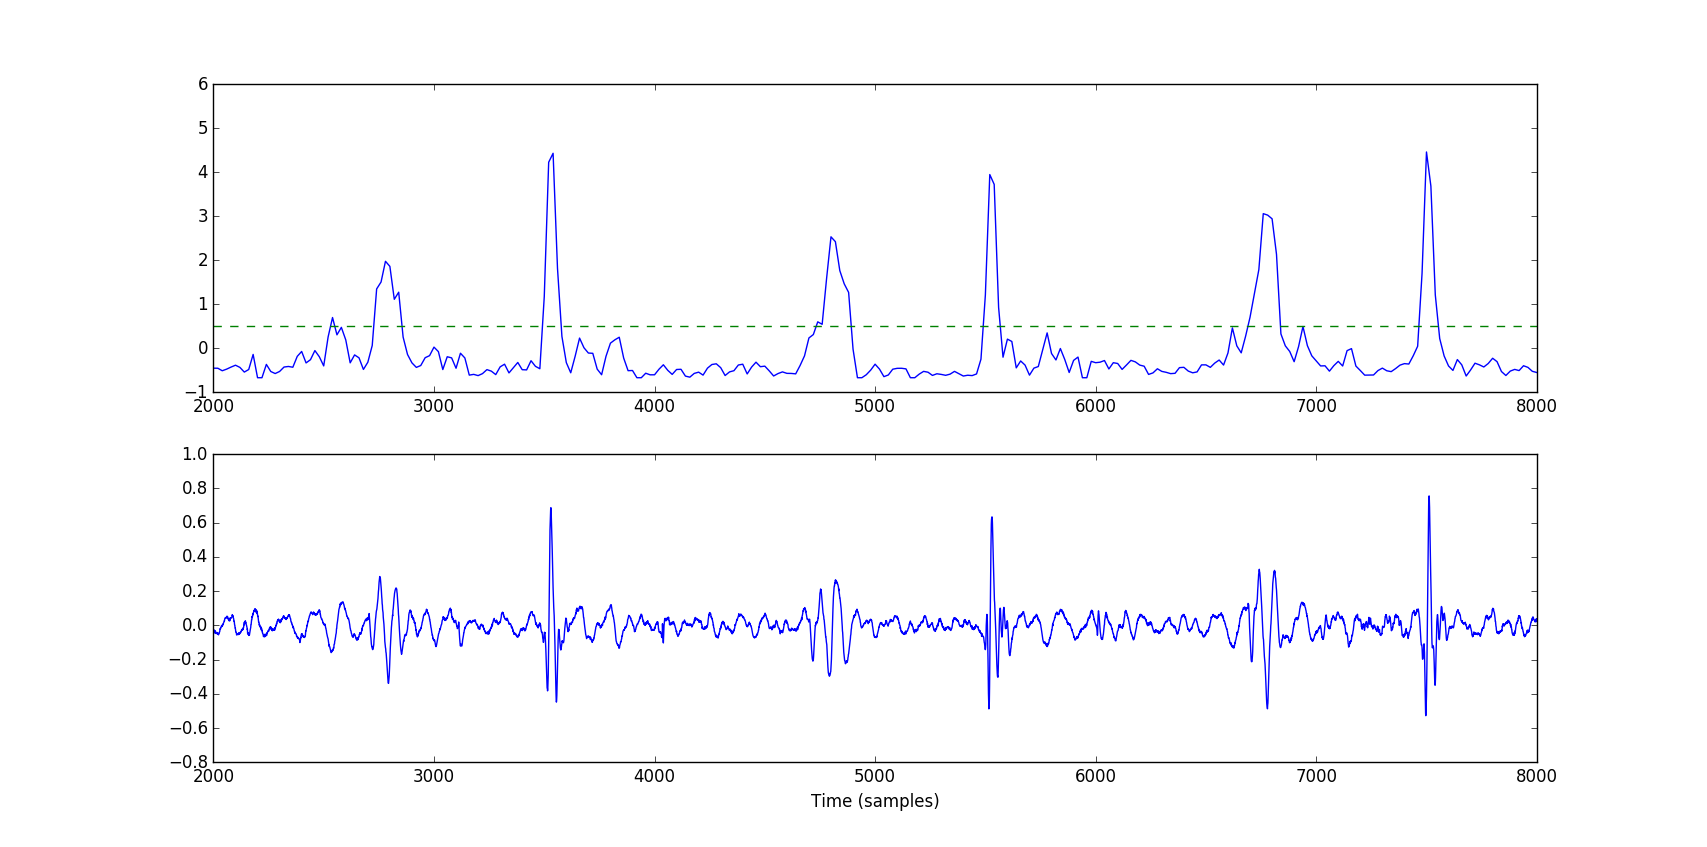
\includegraphics[width=1.1\textwidth]{OfflineShanEngy}}
    \label{OfflineShanEngy}
\end{figure}
\begin{figure}[H]
    \caption{Extra Peak Filtering}
    \makebox[\textwidth]{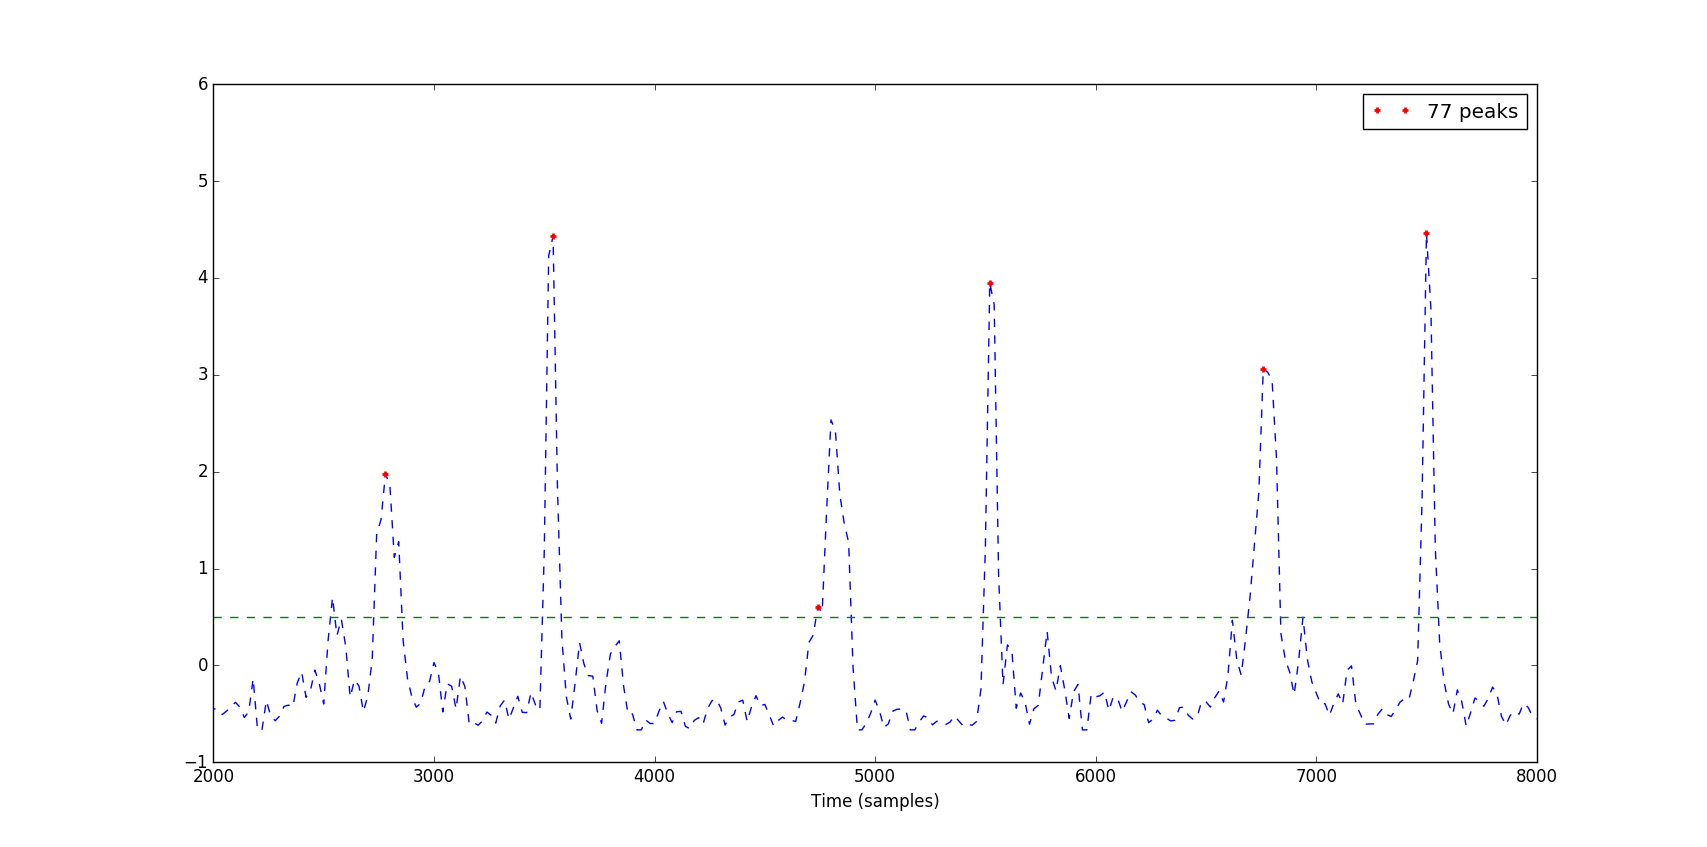
\includegraphics[width=1.1\textwidth]{OfflinePeakFilter}}
    \label{OfflinePeakFilter}
\end{figure}
\begin{figure}[H]
    \caption{Peak Picking}
    \makebox[\textwidth]{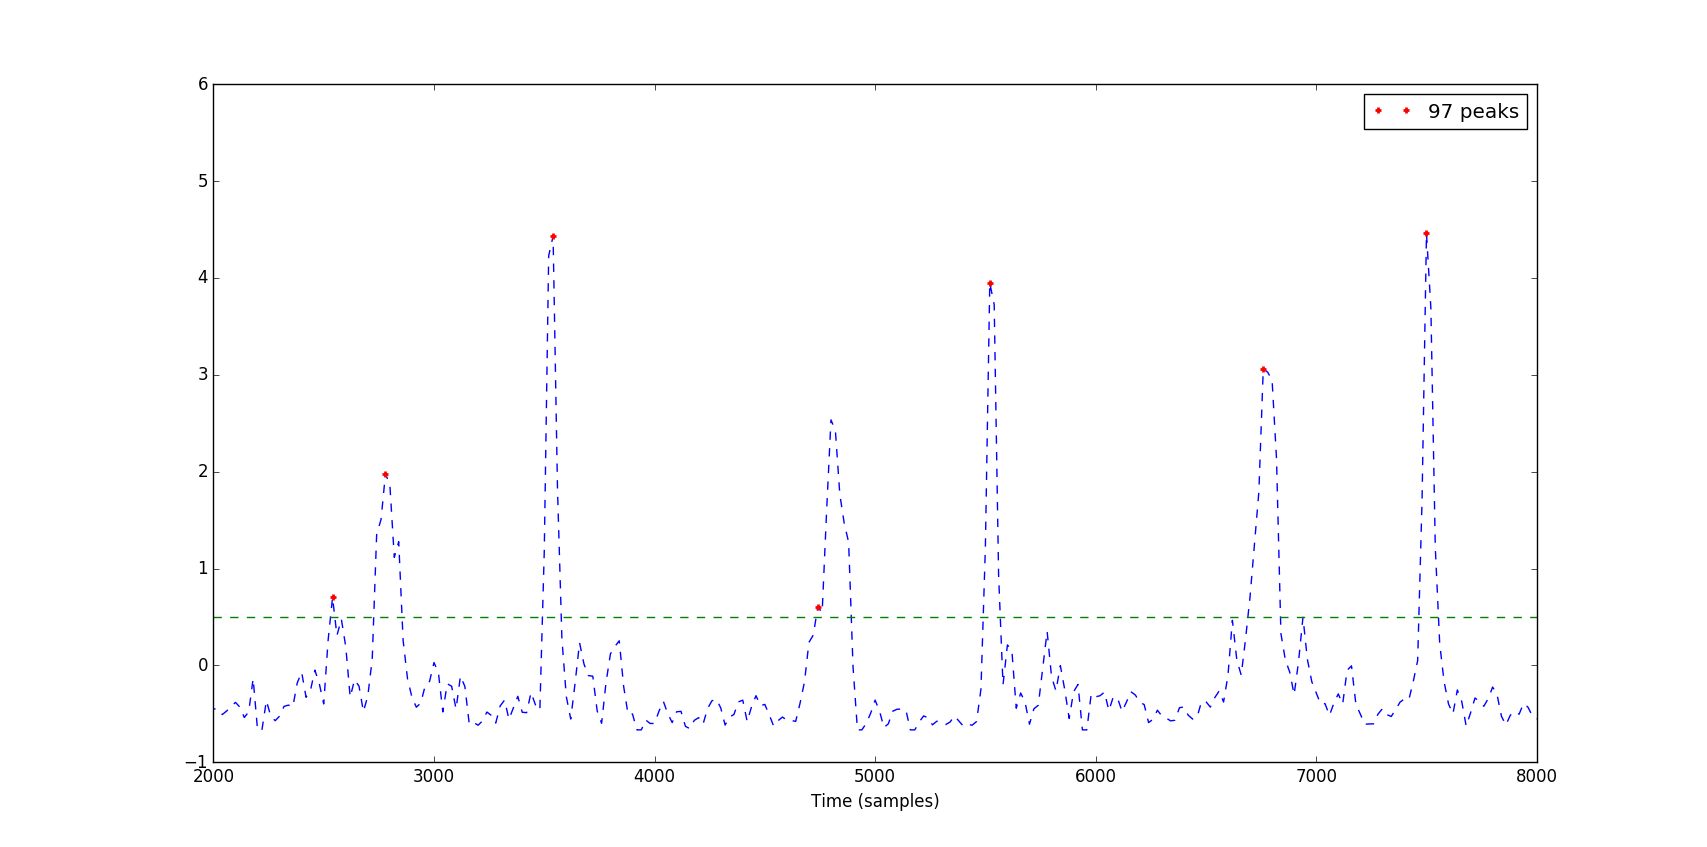
\includegraphics[width=1.1\textwidth]{OfflinePeakPick}}
    \label{OfflinePeakPick}
\end{figure}
\end{document}
